\documentclass{standalone}
\usepackage{tikz, tikz-cd}
\usetikzlibrary{shapes, decorations.markings}
\begin{document}

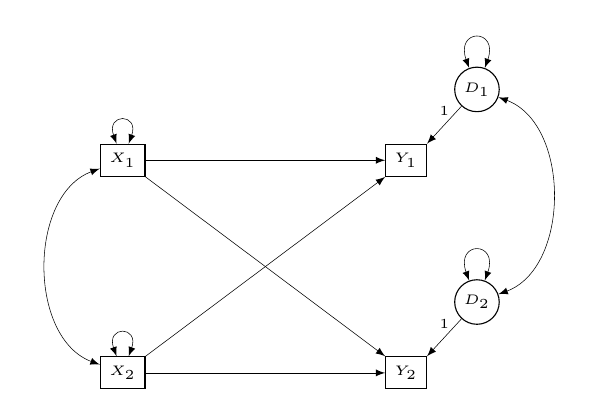
\begin{tikzpicture}[scale=0.9]
\node[draw] (y1) at (5,6) {\tiny{$Y_1$}};
\node[draw] (x1) at (1,6) {\tiny{$X_1$}};
\node[draw] (y2) at (5,3) {\tiny{$Y_2$}};
\node[draw] (x2) at (1,3) {\tiny{$X_2$}};
\node[draw, circle, inner sep=2] (d1) at (6,7) {\tiny{$D_1$}};
\node[draw, circle, inner sep=2] (d2) at (6,4) {\tiny{$D_2$}};
\draw [->, very thin, >=latex] (x1)--(y1.west);
\draw [->, very thin, >=latex] (x2)--(y2.west);
\draw [->, very thin, >=latex] (x1.south east)--(y2.north west);
\draw [->, very thin, >=latex] (x2.north east)--(y1.south west);
\draw [->, very thin, >=latex] (d1)--(y1.north east) node [midway, above] {\tiny{1}};
\draw [->, very thin, >=latex] (d2)--(y2.north east) node [midway, above] {\tiny{1}};
% Residuals:
\draw[<->, very thin, >=latex] (x1) to [out=70,in=110,looseness=7] (x1);
\draw[<->, very thin, >=latex] (x2) to [out=70,in=110,looseness=7] (x2);
\draw[<->, very thin, >=latex] (x1) to [out=200,in=160,looseness=1] (x2);
\draw[<->, very thin, >=latex] (d1) to [out=-20,in=20,looseness=1] (d2);
\draw[<->, very thin, >=latex] (d1) to [out=70,in=110,looseness=7] (d1);
\draw[<->, very thin, >=latex] (d2) to [out=70,in=110,looseness=7] (d2);
\end{tikzpicture}

\end{document}